\subsubsection{英雄机器人}

    \paragraph{规则分析}

        \setlist[itemize]{label=\raisebox{-1.2ex}{\scalebox{3}{$\textbullet$}}}

        \begin{itemize}
            \item 今年的英雄机器人引入了“部署模式”,在己方半场内,英雄机器人可通过2秒的确认时间进入“部署模式”,底盘断电后获得25\%的防御增益,并获得狙击攻击增益与经济加成。这一机制的引入,英雄在己方半场的任意位置,对敌方基地造成可观的伤害输出。“部署模式”需要其他兵种的协同支持,为团队协作和战术规划提供了更多可能性。同时规则对适用于部署模式的“比赛节奏”做出了一些限制,开局有2次命中能享受部署模式加成,此后每20s增加一次机会。
            
            \item 今年新增的42°坡提升了地形复杂度,对英雄机器人的底盘设计和功率分配提出了全新要求。传统的麦克纳姆轮加上英雄机器人的重量难以胜任这一高难度场景,地形上鼓励其他底盘结构(例如舵轮底盘)。42°坡本身是一个极具战略价值的狙击点,占领这里可以对战局产生重要影响。同时这一位置容易受到对方无人机的威胁,对时机的精准把控至关重要。解决这些技术难点,我们就能在比赛中抢占先机,充分释放英雄机器人的潜能。
            
            \item 能量体系:今年的规则更新中,英雄、步兵、哨兵机器人在底盘能量消耗达到20000J后将进入“虚弱”状态,对于比赛节奏和战术规划有新的要求。这一规则也对电容的性能和整车的能量控制系统提出了更高要求。如何提升电容效率、优化整车能量管理,将成为提高胜率的关键技术突破点。
            
            \item 赛制时间分析:在新赛季中,空中支援机制进行了调整,英雄在前30秒需要占领梯形高地、准备击打前哨站,30秒后将与无人机和对方英雄机器人形成制约。地形变化使得梯形高地的防御增益对英雄机器人的吊射和部署模式至关重要。若某方的梯形高地增益点仅被该方机器人占领,则在比赛的不同时间段(2-3分钟、3-5分钟、5-7分钟),占领的机器人可获得2、3、5倍的枪口热量冷却增益和25%的防御增益。
            
            \item 雷达机制分析:雷达可以向所有己方机器人发送数据,接收哨兵机器人的数据。新规则下英雄吊射点位更加灵活,但在部署模式下底盘处于“失能状态”,此时很容易陷入被动。对于吊射的点位,可以通过感知敌方单位位置为英雄操作手标注可以安全进行吊射的位置,或直接检测预设的吊射点位是否有敌方单位,方便操作手进行决策。并在英雄进入部署模式时,感知接近的敌方单位,为操作手提供预警,减少在部署模式下被抓风险,提高灵活性。也可以在敌方进入基地范围内时,向英雄操作手发送"防守"的决策信号,调动英雄回防。

            \item 英雄狙击模式下,命中敌方基地会获得50金币。英雄狙击伤害可获得100经验值,跟上赛季一样,但是区别在于这赛季英雄新增的部署模式,可以随时狙击。也就是说英雄如果能利用好这个狙击能大大增长升级速度,同时前期也可以使用狙击击打较好命中的目标,加速升级。

            \begin{figure}[H]
                \centering
                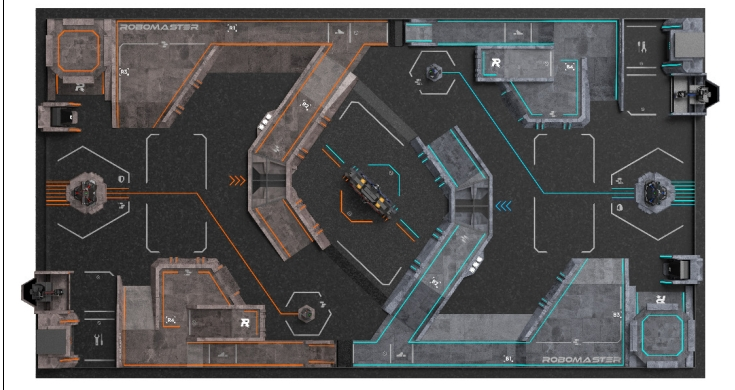
\includegraphics[height=0.35\textwidth]{figure/RM2024_map.png}
                \hspace{0.5em}
                % 添加居中、黑体、加大的字体
                \caption{\textbf{\zihao{-4}\textbf{RM2024场地示意图}}}
                \label{fig:RM2024_map}
            \end{figure}

            
            \begin{figure}[H]
                \centering
                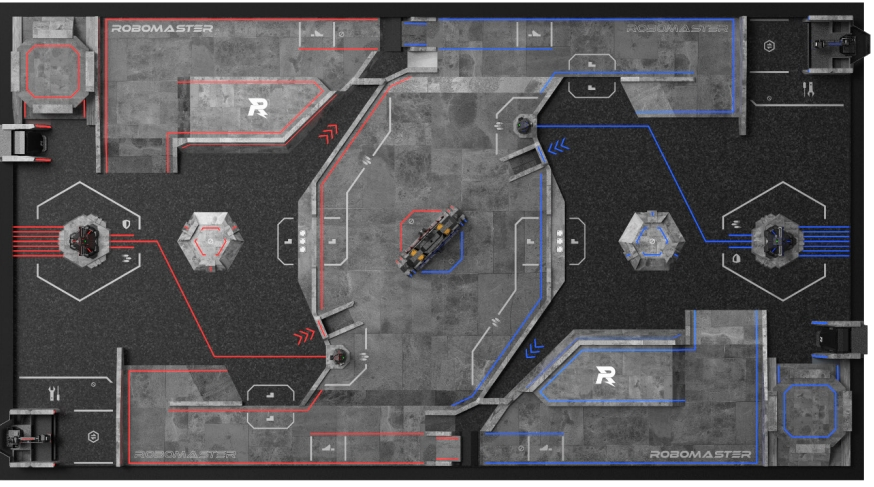
\includegraphics[height=0.35\textwidth]{figure/RM2025_map.png}
                \hspace{0.5em}
                \caption{\textbf{\zihao{-4}\textbf{RM2025场地示意图}}}
                \label{fig:RM2025_map}
            \end{figure}

            \item 场地中央的环形高地也被完全更换为中央高地,进入中央高地的路径也完全更改,24赛季可以由基地区直冲环形高地,但25赛季将公路区和中央高地直接连接,直接阻断了基地区直冲中央高地的想法。这对于英雄的冲锋有十分大的效率影响。并且由于中央高地和梯形高地的改动,导致飞坡后英雄的选择少了一个,这让飞坡风险大大增加,明显要重新考虑飞坡的进攻价值性。

            \item 至于中央高地的20度坡狗洞,和弯曲的香蕉道狭道,对于队内目前英雄而言,无法通过,导致战略意义不大。如果后续场地不加以大的改动,可以尝试制造一台超小英雄过此类狭窄通道。

            \begin{figure}[H]
                \centering
                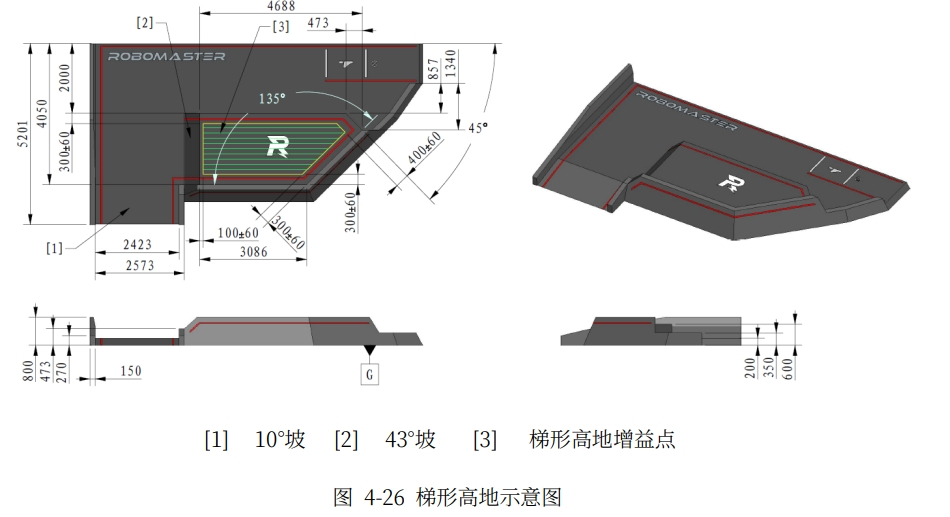
\includegraphics[height=0.35\textwidth]{figure/trapezoidalElevation.png}
                \hspace{0.5em}
                \caption{\textbf{\zihao{-4}\textbf{梯形高地场地示意图}}}
                \label{fig:trapezoidalElevation}
            \end{figure}

            \item 梯形高地最受瞩目的就是那一个43度坡度高地,600的高度让能够上到这个高地的英雄机器人安全性得到了保障,除了平衡步兵或者无人机之外,其他兵种难以构成。此高地还是全场中最适合吊射基地的位置,距离前哨站也只有7~8米的中距离,此间还没有任何的障碍物遮挡视野,功能性一目了然,它就是提供给英雄的专属发射场地,重要性不言而喻。属于英雄前期必需尝试占领的战略要地,并且在前哨站已经攻略了的中期焦灼阶段和后期进攻阶段都可以尝试飞坡占领敌方梯形高地为英雄自己创造一个较为安全的输出基地环境。

            但是对于英雄的性能有一定要求,不管是轮毂影响,还是整个底盘通过角和重心位置设计,对于每一个队伍都是一个大的挑战。
            
            \begin{figure}[H]
                \centering
                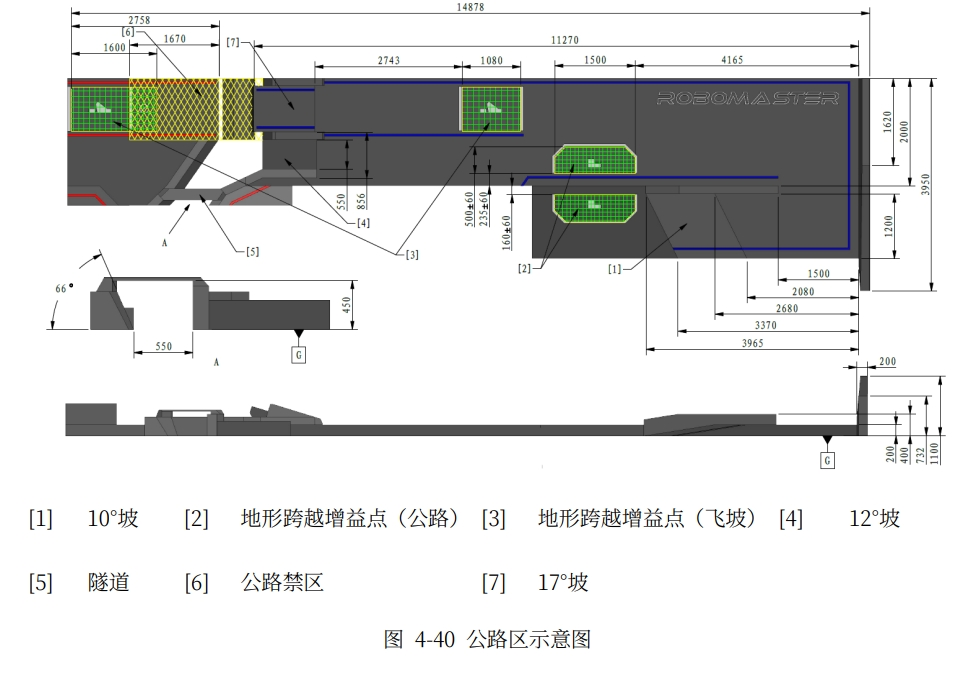
\includegraphics[height=0.35\textwidth]{figure/highwayArea.png}
                \hspace{0.5em}
                \caption{\textbf{\zihao{-4}\textbf{公路区场地示意图}}}
                \label{fig:highwayArea}
            \end{figure}

            \item 对于公路区而言,有台阶増益点,直角弯,飞坡区和,与中央高地衔接的区域。这也是目前对于本队英雄是较优的进攻路径。对于直角弯而言,对于英雄的转弯性能,提出了一个较高的水平要求,对于麦轮底盘和舵轮底盘而言,毫无疑问可以通过,但是对于操作手需要有熟练的要求,减少过弯时间,提高进攻效率。至于飞坡区域,直接衔接到敌方的梯形高地,并且只有梯形高地一条路可以走,一旦被敌方察觉并且派遣车辆堵在梯形高地的出口,那么飞坡过去的英雄只是瓮中之鳖,在战略规划上,若非特别紧急情况不推荐英雄飞坡,但在功能规划上,英雄要具备飞坡功能。最后只剩下与中央高地衔接部分和香蕉道的上坡部分,此地英雄机器人需要注意的是在进攻时段是否有敌方的步兵机器人存在,进攻或撤退时需要保证自身安全,此外没有任何其他过多要求。

            \begin{figure}[H]
                \centering
                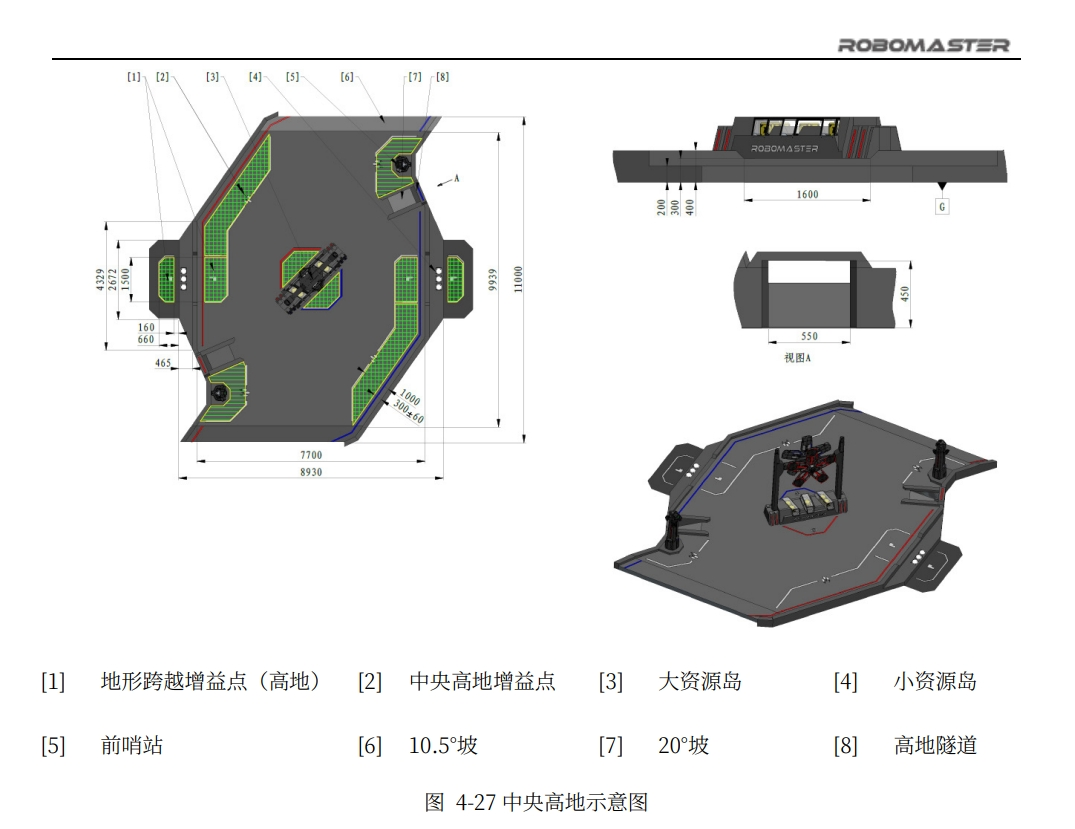
\includegraphics[height=0.35\textwidth]{figure/centralTableland.png}
                \hspace{0.5em}
                \caption{\textbf{\zihao{-4}\textbf{中央高地场地示意图}}}
                \label{fig:centralTableland}
            \end{figure}

            \item 关于中央高地英雄机器人需要注意的就是颠簸路段,敌方“香蕉道”入口,狗洞以及敌方公路区出口。唯一对于车辆性能有要求的就是颠簸路段,尽量减少颠簸对于其影响性,但在多年比赛的经验来看,过颠簸路段时,无法发射,无法防御,只能快速通过,不然只能当活靶子。当英雄机器人在中央高地的时候,一定要时刻注意背后的香蕉道入口,中央高地四通八达前后都有可能面临来敌

        \end{itemize}

        
    
    \paragraph{策略战术}

        \setlist[itemize]{label=\raisebox{-1.2ex}{\scalebox{3}{$\textbullet$}}}

        \begin{itemize}
            \item 出门左拐就是梯形高地了,英雄在比赛开始后可以尝试站住,攻击敌方前哨站,并为己方提供对于中央高地的态势感知。在设想中,梯形高地的落差同时也可为英雄提供对低处攻击的掩蔽,因此这里应该是英雄经常来的地方。
            \item 部署机制以底盘断电为代价换取一系列加成,虽然此时英雄有25\%防御增益,但在潜在的陆空威胁下仍十分脆弱。在地形复杂且四通八达的环境下,要求己方为英雄构建安全的“堡垒地带”显然难度较高,为此英雄操作手应该留意敌方无人机与地面机器人的出动与补给节奏(后半场可能的充电高峰期),见缝插针地抵近输出敌方前哨站与基地,并在危险来临时及时转入防守。
            \item 虽然组委会提过会增加飞坡之后的可选路径,但目前跨过沟壑之后,撤退的路径会经过敌方堡垒区,极有可能一去不复还,从敌方的角度而言飞坡的风险增大了不少。但同时加高的梯形高地也为到达敌方半场的机器人提供了更好的掩体。如果是快结束了想放手一搏可以考虑考虑。
            \item 无论是爬坡上梯形高地还是绕道己方公路区前往中央高地都势必会消耗不少能量,因此英雄应精打细算,增大补给间隔,并在比赛进行到下半场时择机在补给区“充电”。
            \item 对于底盘能量20000J的分配,前期应集中在占领梯形高地,中期寻找不同的部署点攻击对方基地,后期则需退回基地区拦截敌方步兵和英雄.
        \end{itemize}
    
    \paragraph{功能需求分析}

    \LTXtable{\textwidth}{Hero/2.3_functionalRequirement_analysis.tex}
    
    \paragraph{改进方向}

    \LTXtable{\textwidth}{Hero/2.3_improvementDirection.tex}

    \paragraph{研发进度安排}

    \LTXtable{\textwidth}{Hero/2.3_developmentSchedule.tex}

    \paragraph{项目组人员分配}

    \LTXtable{\textwidth}{Hero/2.3_personalAssignment.tex}
    